         \chapter{Classification of matter}
    \setcounter{figure}{1}
    \setcounter{subfigure}{1}
    \label{09a7a4809656be0b739ee130746cd803}
         \section{ Mixtures, compounds and elements}
    \nopagebreak
            \label{m38708} $ \hspace{-5pt}\begin{array}{cccccccccccc}   
\includegraphics[width=0.75cm]{col11305.imgs/summary_fullmarks.png} &   \end{array} $ \hspace{2 pt}\raisebox{-5 pt}{} {(section shortcode: P10011 )} \par 
    \label{m38708*cid1}
            \subsection{ Introduction}
            \nopagebreak
            \label{m38708*id62175}All the objects that we see in the world around us, are made of \textbf{matter}. Matter makes up the air we breathe, the ground we walk on, the food we eat and the animals and plants that live around us. Even our own human bodies are made of matter!\par 
      \label{m38708*id62185}Different objects can be made of different types of matter, or \textbf{materials}. For example, a cupboard (an \textsl{object}) is made of wood, nails and hinges (the \textsl{materials}). The \textbf{properties} of the materials will affect the properties of the object. In the example of the cupboard, the strength of the wood and metals make the cupboard strong and durable. In the same way, the raincoats that you wear during bad weather, are made of a material that is waterproof. The electrical wires in your home are made of metal because metals are a type of material that is able to conduct electricity. It is very important to understand the properties of materials, so that we can use them in our homes, in industry and in other applications. In this chapter, we will be looking at different types of materials and their properties.\par 
\label{m38708*id0132}Some of the properties of matter that you should know are:
\label{m38708*lid825}\begin{itemize}[noitemsep]
            \item Materials can be strong and resist bending (e.g. iron rods, cement) or weak (e.g. fabrics)\item Materials that conduct heat (e.g. metals) are called thermal conductors. Materials that conduct electricity are electrical conductors.\item Brittle materials break easily. Materials that are malleable can be easily formed into different shapes. Ductile materials are able to be formed into long wires.\item Magnetic materials have a magnetic field.\item Density is the mass per unit volume. An example of a dense material is concrete.\item The boiling and melting points of substance help us to classify substances as solids, liquids or gases at a specific temperature.\end{itemize}
\par 
      \label{m38708*id62556}The diagram below shows one way in which matter can be classified (grouped) according to its different properties. As you read further in this chapter, you will see that there are also other ways of classifying materials, for example according to whether or not they are good electrical conductors.\par 
    \setcounter{subfigure}{0}
	\begin{figure}[H] % horizontal\label{m38708*uid1}
    \begin{center}
    \rule[.1in]{\figurerulewidth}{.005in} \\
        \label{m38708*uid1!!!underscore!!!media}\label{m38708*uid1!!!underscore!!!printimage}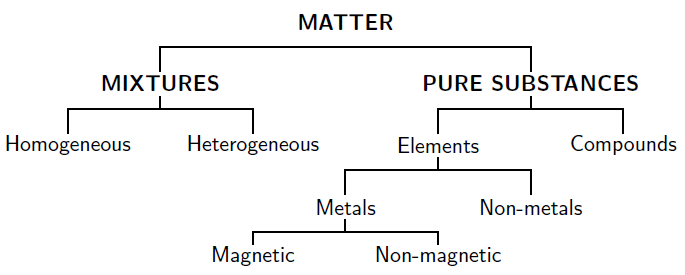
\includegraphics[width=300px]{col11305.imgs/m38708_CG10C1_001.png} % m38708;CG10C1\_001.png;;;6.0;8.5;
      \vspace{2pt}
    \vspace{\rubberspace}\par \begin{cnxcaption}
	  \small \textbf{Figure 1.1: }The classification of matter
	\end{cnxcaption}
    \vspace{.1in}
    \rule[.1in]{\figurerulewidth}{.005in} \\
    \end{center}
 \end{figure}       
    \label{m38708*eip-344}\noindent{}\textbf{Discussion: Everyday materials}In groups of 3 or 4 look at the labels of medicines, food items, and any other items that you use often. What can you tell about the material inside the container from the list of ingredients? Why is it important to have a list of ingredients on the materials that we use? Do some research on the safety data of the various compounds in the items that you looked at. Are the compounds in the items safe to use? In the food items, what preservatives and additives are there? Are these preservatives and additives good for you? Are there natural alternatives (natural alternatives are usually used by indigenous people groups)? \par \label{m38708*cid2}
            \subsection{ Mixtures}
            \nopagebreak
            \label{m38708*id62584}We see mixtures all the time in our everyday lives. A stew, for example, is a mixture of different foods such as meat and vegetables; sea water is a mixture of water, salt and other substances, and air is a mixture of gases such as carbon dioxide, oxygen and nitrogen.\par 
\label{m38708*fhsst!!!underscore!!!id69}\begin{definition}
	  \begin{tabular*}{15 cm}{m{15 mm}m{}}
	\hspace*{-50pt}  
\includegraphics[width=0.5in]{col11305.imgs/psflag2.png}   & \Definition{   \label{id2405672}\textbf{ Mixture }} { \label{m38708*meaningfhsst!!!underscore!!!id69}
      A \textbf{mixture} is a combination of two or more substances, where these substances are not bonded (or joined) to each other. 
       } 
      \end{tabular*}
      \end{definition}
      \label{m38708*id62612}In a mixture, the substances that make up the mixture:\par 
      \label{m38708*id62615}\begin{itemize}[noitemsep]
            \label{m38708*uid2}\item \textsl{are not in a fixed ratio}
Imagine, for example, that you have a 250 ml beaker of water. It doesn't matter whether you add 20 g, 40 g, 100 g or any other mass of sand to the water; it will still be called a mixture of sand and water.
\label{m38708*uid3}\item \textsl{keep their physical properties}
In the example we used of the sand and water, neither of these substances has changed in any way when they are mixed together. Even though the sand is in water, it still has the same properties as when it was out of the water.
\label{m38708*uid4}\item \textsl{can be separated by mechanical means}
To separate something by 'mechanical means', means that there is no chemical process involved. In our sand and water example, it is possible to separate the mixture by simply pouring the water through a filter. Something \textsl{physical} is done to the mixture, rather than something \textsl{chemical}.
\end{itemize}
      \label{m38708*id62689}Some other examples of mixtures include blood (a mixture of blood cells, platelets and plasma), steel (a mixture of iron and other materials) and the gold that is used to make jewellery. The gold in jewellery is not pure gold but is a mixture of metals. The amount of gold in the jewellery is measured in \textsl{karats} (24 karat would be pure gold, while 18 karat is only 75\% gold).\par 
      \label{m38708*id62700}We can group mixtures further by dividing them into those that are heterogeneous and those that are homogeneous.\par 
      \label{m38708*uid5}
            \subsubsection{ Heterogeneous mixtures}
            \nopagebreak
        \label{m38708*id62715}A \textbf{heterogeneous} mixture does not have a definite composition. Think of a pizza, that has a topping of cheese, tomato, mushrooms and peppers (the topping is a mixture). Each slice will probably be slightly different from the next because the toppings (the tomato, cheese, mushrooms and peppers) are not evenly distributed. Another example would be granite, a type of rock. Granite is made up of lots of different mineral substances including quartz and feldspar. But these minerals are not spread evenly through the rock and so some parts of the rock may have more quartz than others. Another example is a mixture of oil and water. Although you may add one substance to the other, they will stay separate in the mixture. We say that these heterogeneous mixtures are \textsl{non-uniform}, in other words they are not exactly the same throughout.\par 
\label{m38708*fhsst!!!underscore!!!id89}\begin{definition}
	  \begin{tabular*}{15 cm}{m{15 mm}m{}}
	\hspace*{-50pt}  
\includegraphics[width=0.5in]{col11305.imgs/psflag2.png}   & \Definition{   \label{id2405839}\textbf{ Heterogeneous mixture }} { \label{m38708*meaningfhsst!!!underscore!!!id89}
        A heterogeneous mixture is one that is non-uniform and the different components of the mixture can be seen.
         } 
      \end{tabular*}
      \end{definition}
      \label{m38708*uid6}
            \subsubsection{ Homogeneous mixtures}
            \nopagebreak
        \label{m38708*id62762}A \textbf{homogeneous} mixture has a definite composition, and specific properties. In a homogeneous mixture, the different parts cannot be seen. A solution of salt dissolved in water is an example of a homogeneous mixture. When the salt dissolves, it will spread evenly through the water so that all parts of the solution are the same, and you can no longer see the salt as being separate from the water. Think also of a powdered drink that you mix with water. Provided you give the container a good shake after you have added the powder to the water, the drink will have the same sweet taste for anyone who drinks it, it won't matter whether they take a sip from the top or from the bottom. The air we breathe is another example of a homogeneous mixture since it is made up of different gases which are in a constant ratio, and which can't be visually distinguished from each other (i.e. you can't see the different components).\par 
\label{m38708*fhsst!!!underscore!!!id96}\begin{definition}
	  \begin{tabular*}{15 cm}{m{15 mm}m{}}
	\hspace*{-50pt}  
\includegraphics[width=0.5in]{col11305.imgs/psflag2.png}   & \Definition{   \label{id2405912}\textbf{ Homogeneous mixture }} { \label{m38708*meaningfhsst!!!underscore!!!id96}
        A homogeneous mixture is one that is uniform, and where the different components of the mixture cannot be seen. 
         } 
      \end{tabular*}
      \end{definition}
        \label{m38708*id62795}An \textbf{alloy} is a homogeneous mixture of two or more elements, at least one of which is a metal, where the resulting material has metallic properties. Alloys are usually made to improve the properties of the elements that make them up. For example steel is much stronger than iron (which is the main component of steel).\par 
\label{m38708*eip-479}\vspace{.5cm} 
      \noindent
      \hspace*{-30pt}
\includegraphics[width=0.5in]{col11305.imgs/pspencil2.png}   \raisebox{25mm}{   
      \begin{mdframed}[linewidth=4, leftmargin=40, rightmargin=40]  
      \begin{exercise}
    \noindent\textbf{Exercise 1.1: Mixtures}\label{m38708*eip-277}
  \label{m38708*eip-353}For each of the following mixtures state whether it is a homogenous or a heterogenous mixture:
\label{m38708*eip-id1167649056231}\begin{enumerate}[noitemsep, label=\textbf{\alph*}. ] 
            \leftskip=20pt\rightskip=\leftskip\item sugar and water\item flour and iron filings (small pieces of iron)\item flour and baking powder\item smarties, jelly tots and peppermints\end{enumerate}
  \par 
\vspace{5pt}
\label{m38708*eip-602}\noindent\textbf{Solution to Exercise }
\label{m38708*eip-id7325184}\begin{enumerate}[noitemsep, label=\textbf{\alph*}. ] 
            \leftskip=20pt\rightskip=\leftskip\item This is a homogenous mixture since we cannot see the sugar in the water. Also, the two components are mixed uniformly.\item This is a heterogenous mixture since we are able to make out the pieces of iron in the flour. In this mixture there may be places where there are a lot of iron filings and places where there is more flour, so it is not uniformly mixed.\item Homogenous mixture since there is no way to distinguish between the flour and the baking powder. The two components of the mixture are uniformly mixed.\item Heterogenous mixture since we can clearly see each of the components that make up the mixture. The three components of the mixture are not evenly distributed.\end{enumerate}
    \end{exercise}
    \end{mdframed}
    }
    \noindent
  \label{m38708*eip-478}\noindent{}\textbf{Activity: Classifying materials}Look around your classroom or school. Make a list of all the different materials that you see around you. Try to work out why a particular material was used. Can you classify all the different materials used according to their properties? On your way to school or at home or in the shops, look at the different materials that are used. Why are these materials chosen over other materials?\par \label{m38708*eip-894}\noindent{}\textbf{Activity: Making mixtures}Make mixtures of sand and water, potassium dichromate and water, iodine and ethanol, iodine and water. Classify these as heterogeneous or homogeneous. Try to make mixtures using other substances. Are the mixtures that you have made heterogeneous or homogeneous? Give reasons for your choice. \par \label{m38708*secfhsst!!!underscore!!!id169}
            \subsubsection{ Mixtures         }
            \nopagebreak
            \label{m38708*id63150}\begin{enumerate}[noitemsep, label=\textbf{\arabic*}. ] 
            \label{m38708*uid17}\item Which of the following substances are \textsl{mixtures}?
\label{m38708*id63170}\begin{enumerate}[noitemsep, label=\textbf{\alph*}. ] 
            \label{m38708*uid18}\item tap water
\label{m38708*uid19}\item brass (an alloy of copper and zinc)
\label{m38708*uid20}\item concrete
\label{m38708*uid21}\item aluminium
\label{m38708*uid22}\item Coca cola
\label{m38708*uid23}\item distilled water
\end{enumerate}
        \label{m38708*uid24}\item In each of the examples above, say whether the mixture is homogeneous or heterogeneous.\newline
     \end{enumerate}
    \label{m38708*cid3}
\par \raisebox{-5 pt}{
\includegraphics[width=0.5cm]{col11305.imgs/summary_www.png}} Find the answers with the shortcodes:
 \par \begin{tabular}[h]{cccccc}
 (1.) llm  & \end{tabular}
            \subsection{ Pure Substances: Elements and Compounds}
            \nopagebreak
      \label{m38708*id63273}Any material that is not a mixture, is called a \textbf{pure substance}. Pure substances include \textbf{elements} and \textbf{compounds}. It is much more difficult to break down pure substances into their parts, and complex chemical methods are needed to do this.\par 
      \label{m38708*eip-862}One way to determine if a substance is pure is to look at its melting or boiling point. Pure substances will have a sharply defined melting or boiling point (i.e. the melting or boiling point will be a single temperature rather than a range of temperatures.) Impure substances have a temperature range over which they melt or boil. We can also use chromatography to determine if a substance is pure or not. Chromatography is the process of separating substances into their individual components. If a substance is pure then chromatography will only produce one substance at the end of the process. If a substance is impure then several substances will be seen at the end of the process. \par \label{m38708*eip-122}\noindent{}\textbf{Activity: Smartie chromatography}You will need filter paper (or chromatography paper), some smarties in different colours, water and an eye dropper. \newline
Place a smartie in the center of a piece of filter paper. Carefully drop a few drops of water onto the smartie. You should see rings of different colour forming around the smartie. Each colour is one of the individual colours that are used to make up the colour of the smartie.\par \label{m38708*eip-392}
\begin{tabular}{cc}
	\hspace*{-50pt}\raisebox{-8 mm}{\hspace{-0.2in}
\includegraphics[width=0.5in]{col11305.imgs/pstip2.png} } & 
	\begin{minipage}{0.85\textwidth}
	\begin{note}
      {note: }For the above activity you can use ordinary filter paper (that is used in coffee filters) from your local store.
	\end{note}
	\end{minipage}
	\end{tabular}
	\par
      \label{m38708*uid25}
            \subsubsection{ Elements}
            \nopagebreak
        \label{m38708*id63302}An \textbf{element} is a chemical substance that can't be divided or changed into other chemical substances by any ordinary chemical means. The smallest unit of an element is the \textbf{atom}.\par 
\label{m38708*fhsst!!!underscore!!!id193}\begin{definition}
	  \begin{tabular*}{15 cm}{m{15 mm}m{}}
	\hspace*{-50pt}  
\includegraphics[width=0.5in]{col11305.imgs/psflag2.png}   & \Definition{   \label{id2406278}\textbf{ Element }} { \label{m38708*meaningfhsst!!!underscore!!!id193}
        An element is a substance that cannot be broken down into other substances through chemical means.
         } 
      \end{tabular*}
      \end{definition}
        \label{m38708*id63334}There are 112 officially named elements and about 118 known elements. Most of these are natural, but some are man-made. The elements we know are represented in the \textbf{Periodic Table of the Elements}, where each element is abbreviated to a \textbf{chemical symbol}. Examples of elements are magnesium ($\mathrm{Mg}$), hydrogen ($\mathrm{H}$), oxygen ($\mathrm{O}$) and carbon ($\mathrm{C}$). On the Periodic Table you will notice that some of the abbreviations do not seem to match the elements they represent. The element iron, for example, has the chemical formula $\mathrm{Fe}$. This is because the elements were originally given Latin names. Iron has the abbreviation $\mathrm{Fe}$ because its Latin name is 'ferrum'. In the same way, sodium's Latin name is 'natrium' ($\mathrm{Na}$) and gold's is 'aurum' ($\mathrm{Au}$).\par \label{m38708*eip-775}
\begin{tabular}{cc}
	\hspace*{-50pt}\raisebox{-8 mm}{\hspace{-0.2in}
\includegraphics[width=0.75in]{col11305.imgs/psfact2.png} } & 
	\begin{minipage}{0.85\textwidth}
	\begin{note}
      {note: }Recently it was agreed that two more elements would be added to the list of officially named elements. These are elements number 114 and 116. The proposed name for element 114 is flerovium and for element 116 it is moscovium. This brings the total number of officially named elements to 114.
	\end{note}
	\end{minipage}
	\end{tabular}
	\par
      \label{m38708*uid26}
            \subsubsection{ Compounds}
            \nopagebreak
        \label{m38708*id63363}A \textbf{compound} is a chemical substance that forms when two or more elements combine in a fixed ratio. Water ($\mathrm{H}{}_{2}\mathrm{O}$), for example, is a compound that is made up of two hydrogen atoms for every one oxygen atom. Sodium chloride ($\mathrm{NaCl}$) is a compound made up of one sodium atom for every chlorine atom. An important characteristic of a compound is that it has a \textbf{chemical formula}, which describes the ratio in which the atoms of each element in the compound occur.\par 
\label{m38708*fhsst!!!underscore!!!id201}\begin{definition}
	  \begin{tabular*}{15 cm}{m{15 mm}m{}}
	\hspace*{-50pt}  
\includegraphics[width=0.5in]{col11305.imgs/psflag2.png}   & \Definition{   \label{id2406453}\textbf{ Compound }} { \label{m38708*meaningfhsst!!!underscore!!!id201}
        A substance made up of two or more elements that are joined together in a fixed ratio.
         } 
      \end{tabular*}
      \end{definition}
        \label{m38708*id63410}Figure~1.2 might help you to understand the difference between the terms \textsl{element}, \textsl{mixture} and \textsl{compound}. Iron (Fe) and sulphur (S) are two elements. When they are added together, they form a \textsl{mixture} of iron and sulphur. The iron and sulphur are not joined together. However, if the mixture is heated, a new \textsl{compound} is formed, which is called iron sulphide (FeS). In this compound, the iron and sulphur are joined to each other in a ratio of 1:1. In other words, one atom of iron is joined to one atom of sulphur in the compound iron sulphide.\par 
    \setcounter{subfigure}{0}
	\begin{figure}[H] % horizontal\label{m38708*uid27}
    \begin{center}
    \rule[.1in]{\figurerulewidth}{.005in} \\
        \label{m38708*uid27!!!underscore!!!media}\label{m38708*uid27!!!underscore!!!printimage}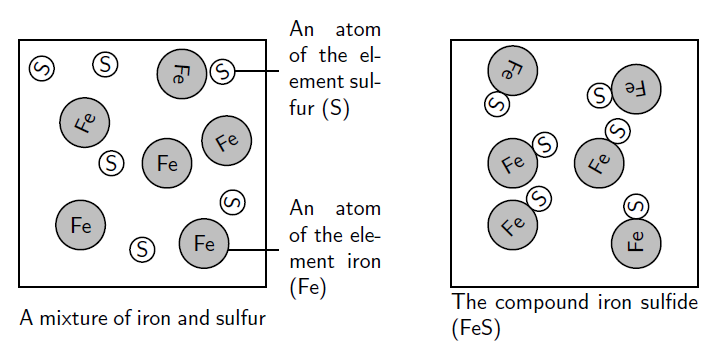
\includegraphics[width=300px]{col11305.imgs/m38708_CG10C1_003.png} % m38708;CG10C1\_003.png;;;6.0;8.5;
      \vspace{2pt}
    \vspace{\rubberspace}\par \begin{cnxcaption}
	  \small \textbf{Figure 1.2: }Understanding the difference between a mixture and a compound
	\end{cnxcaption}
    \vspace{.1in}
    \rule[.1in]{\figurerulewidth}{.005in} \\
    \end{center}
 \end{figure}       
\label{m38708*eip-487}Figure~1.2 shows the microscopic representation of mixtures and compounds. In a microscopic representation we use circles to represent different elements. To show a compound, we draw several circles joined together. Mixtures are simply shown as two or more individual elements in the same box. The circles are not joined for a mixture.\par 
\label{m38708*id0124}We can also use symbols to represent elements, mixtures and compounds. The symbols for the elements are all found on the periodic table. Compounds are shown as two or more element names written right next to each other. Subscripts may be used to show that there is more than one atom of a particular element. (e.g. $\mathrm{H}{}_{2}\mathrm{O}$ or $\mathrm{NaCl}$). Mixtures are written as: a mixture of element (or compound) A and element (or compound) B. (e.g. a mixture of $\mathrm{Fe}$ and $\mathrm{S}$).\par 
\label{m38708*eip-595}One way to think of mixtures and compounds is to think of buildings. The building is a mixture of different building materials (e.g. glass, bricks, cement, etc.). The building materials are all compounds. You can also think of the elements as Lego blocks. Each Lego block can be added to other Lego blocks to make new structures, in the same way that elements can combine to make compounds. \par \label{m38708*eip-524}\vspace{.5cm} 
      \noindent
      \hspace*{-30pt}
\includegraphics[width=0.5in]{col11305.imgs/pspencil2.png}   \raisebox{25mm}{   
      \begin{mdframed}[linewidth=4, leftmargin=40, rightmargin=40]  
      \begin{exercise}
    \noindent\textbf{Exercise 1.2: Mixtures and pure substances}\label{m38708*eip-259}
  \label{m38708*eip-457}
For each of the following substances state whether it is a pure substance or a mixture. If it is a mixture, is it homogenous or heterogenous? If it is a pure substance is it an element or a compound? 
\label{m38708*eip-id1167351497334}\begin{enumerate}[noitemsep, label=\textbf{\alph*}. ] 
            \leftskip=20pt\rightskip=\leftskip\item Blood\item Argon\item Silicon dioxide (${\mathrm{SiO}}_{2}$)\item Sand and stones\end{enumerate}
  \par 
\vspace{5pt}
\label{m38708*eip-62}\noindent\textbf{Solution to Exercise }
\label{m38708*eip-id1167366034146}\begin{enumerate}[noitemsep, label=\textbf{\alph*}. ] 
            \leftskip=20pt\rightskip=\leftskip\item Blood is a mixture since it is made up of many different compounds and substances. Blood is a homogenous mixture since you cannot see the individual components and the components are uniformly distributed.\item Argon is a pure substance. Argon is an element since we can find it on the periodic table.\item Silicon dioxide is a pure substance. It is a compound since it is made of the elements silicon and oxygen joined in a fixed ratio.\item Sand and stones form a mixture. There are two distinct compounds. It is a heterogenous mixture since the particles are not uniformly distributed and we can see the individual pieces.\end{enumerate}
    \end{exercise}
    \end{mdframed}
    }
    \noindent
  \label{m38708*eip-326}\noindent{}\textbf{Activity: Using models to represent substances}Use coloured balls and sticks to represent elements and compounds. Some examples that you can try to build are:
\label{m38708*eip-id1166921187210}\begin{itemize}[noitemsep]
            \item Hydrogen\item Oxygen\item Nitrogen\item Neon\item Sodium chloride (salt, $\mathrm{NaCl}$)\item Potassium permanganate (${\mathrm{KMnO}}_{4}$)\item Water (${\mathrm{H}}_{2}\mathrm{O}$)\item Iron sulphide ($\mathrm{FeS}$)\end{itemize}
Think about the way that we represent substances microscopically. Would you use just one ball to represent an element or many? Why? \par \label{m38708*secfhsst!!!underscore!!!id212}
            \subsubsection{ Elements, mixtures and compounds         }
            \nopagebreak
            \label{m38708*id63472}\begin{enumerate}[noitemsep, label=\textbf{\arabic*}. ] 
            \label{m38708*uid28}\item In the following table, tick whether each of the substances listed is a \textsl{mixture} or a \textsl{pure substance}. If it is a mixture, also say whether it is a homogeneous or heterogeneous mixture.
    % \textbf{m38708*id63499}\par
          \begin{table}[H]
    % \begin{table}[H]
    % \\ 'id2876023' '1'
        \begin{center}
      \label{m38708*id63499}
    \noindent
    \tabletail{%
        \hline
        \multicolumn{3}{|p{\mytableboxwidth}|}{\raggedleft \small \sl continued on next page}\\
        \hline
      }
      \tablelasttail{}
      \begin{xtabular}[t]{|l|l|l|}\hline
        \textbf{Substance} &
        \textbf{Mixture or pure} &
        \textbf{Homogeneous or heterogeneous mixture}% make-rowspan-placeholders
     \tabularnewline\cline{1-1}\cline{2-2}\cline{3-3}
      %--------------------------------------------------------------------
        fizzy colddrink &
         &
        % make-rowspan-placeholders
     \tabularnewline\cline{1-1}\cline{2-2}\cline{3-3}
      %--------------------------------------------------------------------
        steel &
         &
        % make-rowspan-placeholders
     \tabularnewline\cline{1-1}\cline{2-2}\cline{3-3}
      %--------------------------------------------------------------------
        oxygen &
         &
        % make-rowspan-placeholders
     \tabularnewline\cline{1-1}\cline{2-2}\cline{3-3}
      %--------------------------------------------------------------------
        iron filings &
         &
        % make-rowspan-placeholders
     \tabularnewline\cline{1-1}\cline{2-2}\cline{3-3}
      %--------------------------------------------------------------------
        smoke &
         &
        % make-rowspan-placeholders
     \tabularnewline\cline{1-1}\cline{2-2}\cline{3-3}
      %--------------------------------------------------------------------
        limestone (${\mathrm{CaCO}}_{3}$) &
         &
        % make-rowspan-placeholders
     \tabularnewline\cline{1-1}\cline{2-2}\cline{3-3}
      %--------------------------------------------------------------------
    \end{xtabular}
      \end{center}
    \begin{center}{\small\bfseries Table 1.1}\end{center}
    \begin{caption}{\small\bfseries Table 1.1}\end{caption}
\end{table}
    \par
\label{m38708*uid29}\item In each of the following cases, say whether the substance is an element, a mixture or a compound.
\label{m38708*id63912}\begin{enumerate}[noitemsep, label=\textbf{\alph*}. ] 
            \label{m38708*uid30}\item $\mathrm{Cu}$
\label{m38708*uid31}\item iron and sulphur
\label{m38708*uid32}\item $\mathrm{Al}$
\label{m38708*uid33}\item $\mathrm{H}{}_{2}\mathrm{SO}{}_{4}$\label{m38708*uid34}\item $\mathrm{SO}{}_{3}$\end{enumerate}
                \end{enumerate}
    \label{m38708*cid4}
\par \raisebox{-5 pt}{
\includegraphics[width=0.5cm]{col11305.imgs/summary_www.png}} Find the answers with the shortcodes:
 \par \begin{tabular}[h]{cccccc}
 (1.) lly  &  (2.) llV  & \end{tabular}
            \subsection{ Giving names and formulae to substances}
            \nopagebreak
      \label{m38708*eip-379}Think about what you call your friends. Their full name is like the substances name and their nickname is like the substances formulae. Without these names your friends would have no idea which of them you are referring to. In the same way scientists like to have a consistent way of naming things and a short way of describing the thing being named. This helps scientists to communicate efficiently.     \par \label{m38708*id64028}It is easy to describe elements and mixtures. We simply use the names that we find on the periodic table for elements and we use words to describe mixtures. But how are compounds named? In the example of iron sulphide that was used earlier, which element is named first, and which 'ending' is given to the compound name (in this case, the ending is -ide)? \par 
      \label{m38708*id64033}The following are some guidelines for naming compounds:\par 
      \label{m38708*id64037}\begin{enumerate}[noitemsep, label=\textbf{\arabic*}. ] 
            \label{m38708*uid35}\item The compound name will always include the \textbf{names of the elements} that are part of it.
\label{m38708*id64059}\begin{itemize}[noitemsep]
            \label{m38708*uid36}\item A compound of \textbf{iron} ($\mathrm{Fe}$) and \textsl{sulphur} ($\mathrm{S}$) is \textbf{iron}\hspace{1ex}\textsl{sulph}ide ($\mathrm{FeS}$)
\label{m38708*uid37}\item A compound of \textbf{potassium} ($\mathrm{K}$) and \textsl{bromine} ($\mathrm{Br}$) is \textbf{potassium}\hspace{1ex}\textsl{brom}ide ($\mathrm{KBr}$)
\label{m38708*uid38}\item A compound of \textbf{sodium} ($\mathrm{Na}$) and \textsl{chlorine} ($\mathrm{Cl}$) is \textbf{sodium}\hspace{1ex}\textsl{chlor}ide ($\mathrm{NaCl}$)
\end{itemize}
        \label{m38708*uid39}\item In a compound, the element that is on the left of the Periodic Table, is used \textsl{first} when naming the compound. In the example of $\mathrm{NaCl}$, sodium is a group 1 element on the left hand side of the table, while chlorine is in group 7 on the right of the table. Sodium therefore comes first in the compound name. The same is true for $\mathrm{FeS}$ and $\mathrm{KBr}$.
\label{m38708*uid40}\item The \textbf{symbols} of the elements can be used to represent compounds e.g. $\mathrm{FeS}$, $\mathrm{NaCl}$, $\mathrm{KBr}$ and $\mathrm{H}{}_{2}\mathrm{O}$. These are called \textbf{chemical formulae}. In the first three examples, the ratio of the elements in each compound is 1:1. So, for $\mathrm{FeS}$, there is one atom of iron for every atom of sulphur in the compound. In the last example ($\mathrm{H}{}_{2}\mathrm{O}$) there are two atoms of hydrogen for every atom of oxygen in the compound.
\label{m38708*uid41}\item A compound may contain \textbf{compound ions}. An ion is an atom that has lost (positive ion) or gained (negative ion) electrons. Some of the more common compound ions and their formulae are given below.
    % \textbf{m38708*id64235}\par
          \begin{table}[H]
    % \begin{table}[H]
    % \\ 'id2876536' '1'
        \begin{center}
      \label{m38708*id64235}
    \noindent
    \tabletail{%
        \hline
        \multicolumn{2}{|p{\mytableboxwidth}|}{\raggedleft \small \sl continued on next page}\\
        \hline
      }
      \tablelasttail{}
      \begin{xtabular}[t]{|l|l|}\hline
        Name of compound ion &
        Formula% make-rowspan-placeholders
     \tabularnewline\cline{1-1}\cline{2-2}
      %--------------------------------------------------------------------
        Carbonate &
        $\mathrm{CO}_{3}^{2-}$ % make-rowspan-placeholders
     \tabularnewline\cline{1-1}\cline{2-2}
      %--------------------------------------------------------------------
        Sulphate &
         $\mathrm{SO}_{4}^{2-}$% make-rowspan-placeholders
     \tabularnewline\cline{1-1}\cline{2-2}
      %--------------------------------------------------------------------
        Hydroxide &
        ${\mathrm{OH}}^{-}$% make-rowspan-placeholders
     \tabularnewline\cline{1-1}\cline{2-2}
      %--------------------------------------------------------------------
        Ammonium &
        $\mathrm{NH}_{4}^{+}$% make-rowspan-placeholders
     \tabularnewline\cline{1-1}\cline{2-2}
      %--------------------------------------------------------------------
        Nitrate &
        $\mathrm{NO}_{3}^{-}$% make-rowspan-placeholders
     \tabularnewline\cline{1-1}\cline{2-2}
      %--------------------------------------------------------------------
        Hydrogen carbonate &
        $\mathrm{HCO}_{3}^{-}$% make-rowspan-placeholders
     \tabularnewline\cline{1-1}\cline{2-2}
      %--------------------------------------------------------------------
        Phosphate &
        $\mathrm{PO}_{4}^{3-}$% make-rowspan-placeholders
     \tabularnewline\cline{1-1}\cline{2-2}
      %--------------------------------------------------------------------
        Chlorate &
        $\mathrm{ClO}_{3}^{-}$% make-rowspan-placeholders
     \tabularnewline\cline{1-1}\cline{2-2}
      %--------------------------------------------------------------------
        Cyanide &
        ${\mathrm{CN}}^{-}$% make-rowspan-placeholders
     \tabularnewline\cline{1-1}\cline{2-2}
      %--------------------------------------------------------------------
        Chromate &
        $\mathrm{CrO}_{4}^{2-}$% make-rowspan-placeholders
     \tabularnewline\cline{1-1}\cline{2-2}
      %--------------------------------------------------------------------
        Permanganate &
        $\mathrm{MnO}_{4}^{-}$% make-rowspan-placeholders
     \tabularnewline\cline{1-1}\cline{2-2}
      %--------------------------------------------------------------------
    \end{xtabular}
      \end{center}
    \begin{center}{\small\bfseries Table 1.2}\end{center}
    \begin{caption}{\small\bfseries Table 1.2}\end{caption}
\end{table}
    \par
  \label{m38708*uid42}\item When there are only two elements in the compound, the compound is often given a \textbf{suffix} (ending) of -ide. You would have seen this in some of the examples we have used so far. For compound ions, when a non-metal is combined with oxygen to form a negative ion (anion) which then combines with a positive ion (cation) from hydrogen or a metal, then the suffix of the name will be ...ate or ...ite. $\mathrm{NO}_{3}^{-}$ for example, is a negative ion, which may combine with a cation such as hydrogen ($\mathrm{HNO}{}_{3}$) or a metal like potassium (KNO$_\text{3}$). The $\mathrm{NO}_{3}^{-}$ anion has the name nitr\textbf{ate}. $\mathrm{SO}_{3}^{2-}$ in a formula is sulph\textbf{ite}, e.g. sodium sulphite ($\mathrm{Na}{}_{2}\mathrm{SO}{}_{3}$).\newline
     $\mathrm{SO}_{4}^{2-}$ is sulph\textbf{ate} and $\mathrm{PO}_{4}^{3-}$ is phosph\textbf{ate}.
\label{m38708*uid43}\item \textbf{Prefixes} can be used to describe the ratio of the elements that are in the compound. You should know the following prefixes: 'mono' (one), 'di' (two) and 'tri' (three).
\label{m38708*id64977}\begin{itemize}[noitemsep]
            \label{m38708*uid44}\item $\mathrm{CO}$ (carbon monoxide) - There is one atom of oxygen for every one atom of carbon
\label{m38708*uid45}\item $\mathrm{NO}{}_{2}$ (nitrogen dioxide) - There are two atoms of oxygen for every one atom of nitrogen
\label{m38708*uid46}\item $\mathrm{SO}{}_{3}$ (sulphur trioxide) - There are three atoms of oxygen for every one atom of sulphur
\end{itemize}
        \end{enumerate}
\label{m38708*id537402}The above guidelines also help us to work out the formula of a compound from the name of the compound.\par 
\label{m38708*eip-178}When working out the formula of a compound from the name we work backwards. For example, if you are given potassium chloride and were told to give its formula you would start by noting that we having potassium and chloride. Next you write down the formula for each of these ions. Potassium is ${\mathrm{K}}^{+}$ and chloride is ${\mathrm{Cl}}^{-}$. The final step is to note the charge on each ion to see how it combines. Since both potassium and chlorine have a charge of 1, they combine in a 1:1 ratio. The formula is $\mathrm{KCl}$.\par \label{m38708*notfhsst!!!underscore!!!id252}
\begin{tabular}{cc}
	   \hspace*{-50pt}\raisebox{-8 mm}{ 
\includegraphics[width=0.5in]{col11305.imgs/pstip2.png}  }& 
	\begin{minipage}{0.85\textwidth}
	\begin{note}
      {tip: }
      \label{m38708*id65053}When numbers are written as 'subscripts' in compounds (i.e. they are written below and to the right of the element symbol), this tells us how many atoms of that element there are in relation to other elements in the compound. For example in nitrogen dioxide (${\mathrm{NO}}_{2}$) there are two oxygen atoms for every one atom of nitrogen. In sulphur trioxide (${\mathrm{SO}}_{3}$), there are three oxygen atoms for every one atom of sulphur in the compound. Later, when we start looking at chemical equations, you will notice that sometimes there are numbers \textsl{before} the compound name. For example, $2\mathrm{H}{}_{2}\mathrm{O}$ means that there are two molecules of water, and that in each molecule there are two hydrogen atoms for every one oxygen atom. \par  
	\end{note}
	\end{minipage}
	\end{tabular}
	\par
\label{m38708*eip-163}We can use these rules to help us name both ionic compounds and covalent compounds (more on these compounds will be covered in a later chapter). However, covalent compounds are often given other names by scientists to simplify the name (or because the molecule was named long before its formula was discovered). For example, if we have 2 hydrogen atoms and one oxygen atom the above naming rules would tell us that the substance is dihydrogen monoxide. But this compound is better known as water! Or if we had 1 carbon atom and 4 hydrogen atoms then the name would be carbon tetrahydride, but scientists call this compound methane.  \par \label{m38708*eip-254}\vspace{.5cm} 
      \noindent
      \hspace*{-30pt}
\includegraphics[width=0.5in]{col11305.imgs/pspencil2.png}   \raisebox{25mm}{   
      \begin{mdframed}[linewidth=4, leftmargin=40, rightmargin=40]  
      \begin{exercise}
    \noindent\textbf{Exercise 1.3: Naming compounds}\label{m38708*eip-671}
  \label{m38708*eip-870}
    What is the chemical name for \label{m38708*id734}\begin{enumerate}[noitemsep, label=\textbf{\alph*}. ] 
            \leftskip=20pt\rightskip=\leftskip\item  
 $\mathrm{K}{\mathrm{MnO}}_{4}$\item ${\mathrm{NH}}_{4}Cl$\end{enumerate}
  \par 
\vspace{5pt}
\label{m38708*eip-824}\noindent\textbf{Solution to Exercise }
\label{m38708*id7432}\begin{enumerate}[noitemsep, label=\textbf{Step} \textbf{\arabic*}. ] 
            \leftskip=20pt\rightskip=\leftskip\item For a) we have potassium and the permanganate ion. For b) we have the ammonium ion and chlorine. 
\item For a) we list the potassium first and the permanganate ion second. So a) is potassium permanganate. For b) we list the ammonium ion first and change the ending of chlorine to -ide. So b) is ammonium chloride.
\end{enumerate}
    \end{exercise}
    \end{mdframed}
    }
    \noindent
  \par
            \label{m38708*eip-530}\vspace{.5cm} 
      \noindent
      \hspace*{-30pt}
\includegraphics[width=0.5in]{col11305.imgs/pspencil2.png}   \raisebox{25mm}{   
      \begin{mdframed}[linewidth=4, leftmargin=40, rightmargin=40]  
      \begin{exercise}
    \noindent\textbf{Exercise 1.4}\label{m38708*eip-196}
  \label{m38708*eip-535}Write the chemical formulae for: 
\label{m38708*id87432}\begin{enumerate}[noitemsep, label=\textbf{\alph*}. ] 
            \leftskip=20pt\rightskip=\leftskip\item sodium sulphate\item potassium chromate\end{enumerate}
  \par 
\vspace{5pt}
\label{m38708*eip-345}\noindent\textbf{Solution to Exercise }
\label{m38708*id874452}\begin{enumerate}[noitemsep, label=\textbf{Step} \textbf{\arabic*}. ] 
            \leftskip=20pt\rightskip=\leftskip\item In part a) we have ${Na}^{+}$ (sodium) and $\mathrm{SO}_{4}^{2-}$ (sulphate). In part b) we have ${\mathrm{K}}^{+}$ (potassium) and $\mathrm{CrO}_{4}^{2-}$ (chromate)\item In part a) the charge on sodium is $+1$ and the charge on sulphate is $-2$, so we must have two sodiums for every sulphate. In part b) the charge on potassium is $+1$ and the charge on chromate is $-2$, so we must have two potassiums for every chromate.\item a) is ${Na}_{2}{\mathrm{SO}}_{4}$ and b) is ${\mathrm{K}}_{2}{\mathrm{CrO}}_{4}$\end{enumerate}
    \end{exercise}
    \end{mdframed}
    }
    \noindent
  \label{m38708*secfhsst!!!underscore!!!id255}
            \subsubsection{  Naming compounds
      }
            \nopagebreak
      \label{m38708*id65118}\begin{enumerate}[noitemsep, label=\textbf{\arabic*}. ] 
            \label{m38708*uid47}\item The formula for calcium carbonate is $\mathrm{CaCO}{}_{3}$.
\label{m38708*id65148}\begin{enumerate}[noitemsep, label=\textbf{\alph*}. ] 
            \label{m38708*uid48}\item Is calcium carbonate a mixture or a compound? Give a reason for your answer.
\label{m38708*uid49}\item What is the ratio of $Ca:\mathrm{C}:\mathrm{O}$ atoms in the formula?
\end{enumerate}
\label{m38708*uid50}\item Give the name of each of the following substances.
\label{m38708*id65189}\begin{enumerate}[noitemsep, label=\textbf{\alph*}. ] 
            \label{m38708*uid51}\item $\mathrm{KBr}$
\label{m38708*uid52}\item $\mathrm{HCl}$
\label{m38708*uid53}\item ${\mathrm{KMnO}}_{4}$\label{m38708*uid54}\item ${\mathrm{NO}}_{2}$\label{m38708*uid55}\item ${\mathrm{NH}}_{4}\mathrm{OH}$
\label{m38708*uid56}\item ${Na}_{2}{\mathrm{SO}}_{4}$\end{enumerate}
\label{m38708*uid57}\item Give the chemical formula for each of the following compounds.
\label{m38708*id65338}\begin{enumerate}[noitemsep, label=\textbf{\alph*}. ] 
            \label{m38708*uid58}\item potassium nitrate
\label{m38708*uid59}\item sodium iodide
\label{m38708*uid60}\item barium sulphate
\label{m38708*uid61}\item nitrogen dioxide
\label{m38708*uid62}\item sodium monosulphate
\end{enumerate}
\label{m38708*uid63}\item Refer to the diagram below, showing sodium chloride and water, and then answer the questions that follow.
    \setcounter{subfigure}{0}
	\begin{figure}[H] % horizontal\label{m38708*id65419}
    \begin{center}
    \label{m38708*id65419!!!underscore!!!media}\label{m38708*id65419!!!underscore!!!printimage}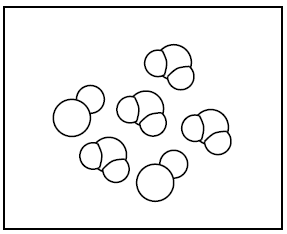
\includegraphics[width=4cm]{col11305.imgs/m38708_CG10C1_004.png} % m38708;CG10C1\_004.png;;;6.0;8.5;
      \vspace{2pt}
    \vspace{.1in}
    \end{center}
 \end{figure}       \label{m38708*id65426}\begin{enumerate}[noitemsep, label=\textbf{\alph*}. ] 
            \label{m38708*uid64}\item What is the chemical formula for water?
\label{m38708*uid65}\item What is the chemical formula for sodium chloride?
\label{m38708*uid66}\item Label the water and sodium chloride in the diagram.
\label{m38708*uid67}\item Give a description of the picture. Focus on whether there are elements or compounds and if it is a mixture or not.
\end{enumerate}
\end{enumerate}
    \label{m38708*cid5}
\par \raisebox{-5 pt}{
\includegraphics[width=0.5cm]{col11305.imgs/summary_www.png}} Find the answers with the shortcodes:
 \par \begin{tabular}[h]{cccccc}
 (1.) llp  &  (2.) lld  &  (3.) llv  &  (4.) llL  & \end{tabular}
            \subsection{ Metals, Metalloids and Non-metals}
            \nopagebreak
      \label{m38708*id65693}The elements in the Periodic Table can also be divided according to whether they are \textbf{metals}, \textbf{metalloids} or \textbf{non-metals}. On the right hand side of the Periodic Table you can draw a 'zigzag' line (This line starts with Boron ($\mathrm{B}$) and goes down to Polonium ($Po$). This line separates all the elements that are metals from those that are non-metals. Metals are found on the left of the line, and non-metals are those on the right. Along the line you find the metalloids. You should notice that there are more metals then non-metals. Metals, metalloids and non-metals all have their own specific properties.\par 
      \label{m38708*uid76}
            \subsubsection{ Metals}
            \nopagebreak
        \label{m38708*id65726}Examples of metals include copper ($Cu$), zinc ($Zn$), gold ($Au$), silver ($Ag$), tin ($Sn$) and lead($Pb$). On the Periodic Table, the metals are on the left of the zig-zag line. There are a large number of elements that are metals. The following are some of the properties of metals:\par 
        \label{m38708*id65732}\begin{itemize}[noitemsep]
            \label{m38708*uid77}\item \textsl{Thermal conductors}
Metals are good conductors of heat. This makes them useful in cooking utensils such as pots and pans.
\label{m38708*uid78}\item \textsl{Electrical conductors}
Metals are good conductors of electricity. Metals can be used in electrical conducting wires.
\label{m38708*uid79}\item \textsl{Shiny metallic lustre}
Metals have a characteristic shiny appearance and so are often used to make jewellery.
\label{m38708*uid80}\item \textsl{Malleable}
This means that they can be bent into shape without breaking.
\label{m38708*uid81}\item \textsl{Ductile}
Metals (such as copper) can be stretched into thin wires, which can then be used to conduct electricity, as well as for other uses.
\label{m38708*uid82}\item \textsl{Melting point}
Metals usually have a high melting point and can therefore be used to make cooking pots and other equipment that needs to become very hot, without being damaged.
\end{itemize}
        \label{m38708*id65852}You can see how the properties of metals make them very useful in certain applications.\par 
\label{m38708*secfhsst!!!underscore!!!id320}
            \subsubsection{  Group Work : Looking at metals
        }
            \nopagebreak
        \label{m38708*id65869}\begin{enumerate}[noitemsep, label=\textbf{\arabic*}. ] 
            \label{m38708*uid83}\item Collect a number of metal items from your home or school. Some examples are listed below:
\label{m38708*id65885}\begin{itemize}[noitemsep]
            \label{m38708*uid84}\item hammer
\label{m38708*uid85}\item wire
\label{m38708*uid86}\item cooking pots
\label{m38708*uid87}\item jewellery
\label{m38708*uid88}\item nails
\label{m38708*uid89}\item coins
\end{itemize}
        \label{m38708*uid90}\item In groups of 3-4, combine your collection of metal objects.
\label{m38708*uid91}\item What is the function of each of these objects?
\label{m38708*uid92}\item Discuss why you think metal was used to make each object. You should consider the properties of metals when you answer this question.
\end{enumerate}
      \label{m38708*uid93}
            \subsubsection{ Non-metals}
            \nopagebreak
        \label{m38708*id66021}In contrast to metals, non-metals are poor thermal conductors, good electrical insulators (meaning that they do \textsl{not} conduct electrical charge) and are neither malleable nor ductile. The non-metals are found on the right hand side of the Periodic Table, and include elements such as sulphur ($\mathrm{S}$), phosphorus ($\mathrm{P}$), nitrogen ($\mathrm{N}$) and oxygen ($\mathrm{O}$).\par 
      \label{m38708*uid94}
            \subsubsection{ Metalloids}
            \nopagebreak
        \label{m38708*id66042}Metalloids or semi-metals have mostly non-metallic properties. One of their distinguishing characteristics is that their conductivity increases as their temperature increases. This is the opposite of what happens in metals. This property is known as semi-conductance and the materials are called semi-conductors. Semi-conductors are important in digital electronics, such as computers. The metalloids include elements such as silicon ($\mathrm{Si}$) and germanium ($\mathrm{Ge}$). Notice where these elements are positioned in the Periodic Table.\par 
      \label{m38708*eip-690}You should now be able to take any material and determine whether it is a metal, non-metal or metalloid simply by using its properties. \par \label{m38708*eip-586}\vspace{.5cm} 
      \noindent
      \hspace*{-30pt}
\includegraphics[width=0.5in]{col11305.imgs/pspencil2.png}   \raisebox{25mm}{   
      \begin{mdframed}[linewidth=4, leftmargin=40, rightmargin=40]  
      \begin{exercise}
    \noindent\textbf{Exercise 1.5: Metals, metalloids and non-metals 1}\label{m38708*eip-77}
  \label{m38708*eip-252}
For each of the following substances state whether they are metals, metalloids or non-metals, using their position on the periodic table.
\label{m38708*eip-id1170734629720}\begin{enumerate}[noitemsep, label=\textbf{\alph*}. ] 
            \leftskip=20pt\rightskip=\leftskip\item Oxygen\item Arsenic\item Vanadium\item Potassium\end{enumerate}
  \par 
\vspace{5pt}
\label{m38708*eip-149}\noindent\textbf{Solution to Exercise }
\label{m38708*eip-id1170750216596}\begin{enumerate}[noitemsep, label=\textbf{\alph*}. ] 
            \leftskip=20pt\rightskip=\leftskip\item Oxygen is on the right of the zigzag line and so is a non-metal.\item Arsenic is on the zigzag line and is a metalloid.\item Vandaium is on the left of zigzag line and so is a metal.\item Potassium is on the left of the zigzag line and so is a metal.\end{enumerate}
    \end{exercise}
    \end{mdframed}
    }
    \noindent
  \par
            \label{m38708*eip-173}\vspace{.5cm} 
      \noindent
      \hspace*{-30pt}
\includegraphics[width=0.5in]{col11305.imgs/pspencil2.png}   \raisebox{25mm}{   
      \begin{mdframed}[linewidth=4, leftmargin=40, rightmargin=40]  
      \begin{exercise}
    \noindent\textbf{Exercise 1.6: Metals, metalloids and non-metals 2}\label{m38708*eip-757}
  \label{m38708*eip-25442}For each of the following substances state whether they are metals, metalloids or non-metals, using the information given.
\label{m38708*eip-id1170742635239}\begin{enumerate}[noitemsep, label=\textbf{\alph*}. ] 
            \leftskip=20pt\rightskip=\leftskip\item Aluminium in a cooking pot\item Silicon in a computer chip\item Plastic insulation around a wire\item Silver jewellery\end{enumerate}
  \par 
\vspace{5pt}
\label{m38708*eip-1455}\noindent\textbf{Solution to Exercise }
\label{m38708*eip-id1170755988427}\begin{enumerate}[noitemsep, label=\textbf{\alph*}. ] 
            \leftskip=20pt\rightskip=\leftskip\item A cooking pot needs to be able to conduct heat and so the aluminium used must be a metal.\item Computer chips rely on semi-conductors and all metalloids are semiconductors. So silicon is a metalloid.\item The plastic around the wire must be insulating to current and so is a non-metal.\item Silver in the jewellery is chosen for its malleability and shiny lustre. So silver is a metal.\end{enumerate}
    \end{exercise}
    \end{mdframed}
    }
    \noindent
  \label{m38708**end}
         \section{ Properties}
    \nopagebreak
            \label{m38706} $ \hspace{-5pt}\begin{array}{cccccccccccc}   
\includegraphics[width=0.75cm]{col11305.imgs/summary_simulation.png} &   
\includegraphics[width=0.75cm]{col11305.imgs/summary_video.png} &   \end{array} $ \hspace{2 pt}\raisebox{-5 pt}{} {(section shortcode: P10012 )} \par 
    \label{m38706*cid6}
            \subsection{ Electrical conductors, semi-conductors and insulators}
            \nopagebreak
            \label{m38706*id66058}An \textbf{electrical conductor} is a substance that allows an electrical current to pass through it. Electrical conductors are usually metals. \textsl{Copper} is one of the best electrical conductors, and this is why it is used to make conducting wire. In reality, \textsl{silver} actually has an even higher electrical conductivity than copper, but because silver is so expensive, it is not practical to use it for electrical wiring because such large amounts are needed. In the overhead power lines that we see above us, \textsl{aluminium} is used. The aluminium usually surrounds a steel core which adds tensile strength to the metal so that it doesn't break when it is stretched across distances. Occasionally gold is used to make wire, not because it is a particularly good conductor, but because it is very resistant to surface corrosion. \textsl{Corrosion} is when a material starts to deteriorate at the surface because of its reactions with the surroundings, for example oxygen and water in the air.\par 
      \label{m38706*id66098}An \textbf{insulator} is a non-conducting material that does not carry any charge. Examples of insulators would be plastic and wood. Do you understand now why electrical wires are normally covered with plastic insulation? \textbf{Semi-conductors} behave like insulators when they are cold, and like conductors when they are hot. The elements silicon and germanium are examples of semi-conductors.\par 
\label{m38706*fhsst!!!underscore!!!id354}\begin{definition}
	  \begin{tabular*}{15 cm}{m{15 mm}m{}}
	\hspace*{-50pt}  
\includegraphics[width=0.5in]{col11305.imgs/psflag2.png}   & \Definition{   \label{id2409398}\textbf{ Conductors and insulators }} { \label{m38706*meaningfhsst!!!underscore!!!id354}
      \label{m38706*id66124}A conductor allows the easy movement or flow of something such as heat or electrical charge through it. Insulators are the opposite to conductors because they \textsl{inhibit} or reduce the flow of heat, electrical charge, sound etc through them. \par 
       } 
      \end{tabular*}
      \end{definition}
\label{m38706*id0522}Think about the materials around you. Are they electrical conductors or not? Why are different materials used? Think about the use of semiconductors in electronics? Can you think of why they are used there?\par 
\label{m38706*secfhsst!!!underscore!!!id357}
            \subsubsection{ Experiment : Electrical conductivity }
            \nopagebreak
            \label{m38706*id66151}\noindent{}\textbf{Aim:}
        \newline
To investigate the electrical conductivity of a number of substances\par 
      \label{m38706*id66166}\noindent{}\textbf{Apparatus:}
        \newline
      \label{m38706*id66175}\begin{itemize}[noitemsep]
            \label{m38706*uid95}\item two or three cells
\label{m38706*uid96}\item light bulb
\label{m38706*uid97}\item crocodile clips
\label{m38706*uid98}\item wire leads
\label{m38706*uid99}\item a selection of test substances (e.g. a piece of plastic, aluminium can, metal pencil sharpener, magnet, wood, chalk).
\end{itemize}
        \par 
      \label{m38706*id66241}
    \setcounter{subfigure}{0}
	\begin{figure}[H] % horizontal\label{m38706*id66244}
    \begin{center}
    \label{m38706*id66244!!!underscore!!!media}\label{m38706*id66244!!!underscore!!!printimage}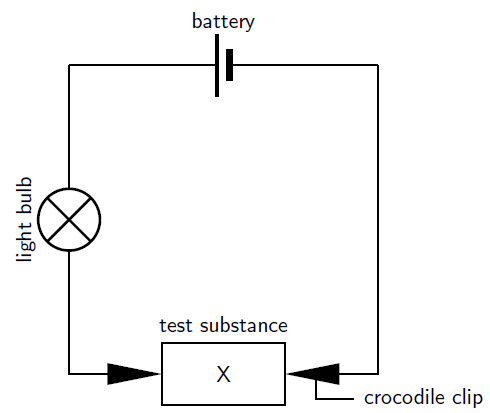
\includegraphics[width=7cm]{col11305.imgs/m38706_CG10C1_006.png} % m38706;CG10C1\_006.png;;;6.0;8.5;
      \vspace{2pt}
    \vspace{.1in}
    \end{center}
 \end{figure}       
      \par 
      \label{m38706*id66251}\noindent{}\textbf{Method:}
        \newline
      \label{m38706*id66260}\begin{enumerate}[noitemsep, label=\textbf{\arabic*}. ] 
            \label{m38706*uid100}\item Set up the circuit as shown above, so that the test substance is held between the two crocodile clips. The wire leads should be connected to the cells and the light bulb should also be connected into the circuit.
\label{m38706*uid101}\item Place the test substances one by one between the crocodile clips and see what happens to the light bulb.
\end{enumerate}
        \par 
      \label{m38706*id66291}\noindent{}\textbf{Results:}
        \newline
      Record your results in the table below:
    % \textbf{m38706*id66304}\par
          \begin{table}[H]
    % \begin{table}[H]
    % \\ '' '0'
        \begin{center}
      \label{m38706*id66304}
    \noindent
    \tabletail{%
        \hline
        \multicolumn{4}{|p{\mytableboxwidth}|}{\raggedleft \small \sl continued on next page}\\
        \hline
      }
      \tablelasttail{}
      \begin{xtabular}[t]{|l|l|l|l|}\hline
                \textbf{Test substance}
               &
                \textbf{Metal/non-metal}
               &
                \textbf{Does the light bulb glow?}
               &
                \textbf{Conductor or insulator}
              % make-rowspan-placeholders
     \tabularnewline\cline{1-1}\cline{2-2}\cline{3-3}\cline{4-4}
      %--------------------------------------------------------------------
         &
         &
         &
        % make-rowspan-placeholders
     \tabularnewline\cline{1-1}\cline{2-2}\cline{3-3}\cline{4-4}
      %--------------------------------------------------------------------
         &
         &
         &
        % make-rowspan-placeholders
     \tabularnewline\cline{1-1}\cline{2-2}\cline{3-3}\cline{4-4}
      %--------------------------------------------------------------------
         &
         &
         &
        % make-rowspan-placeholders
     \tabularnewline\cline{1-1}\cline{2-2}\cline{3-3}\cline{4-4}
      %--------------------------------------------------------------------
         &
         &
         &
        % make-rowspan-placeholders
     \tabularnewline\cline{1-1}\cline{2-2}\cline{3-3}\cline{4-4}
      %--------------------------------------------------------------------
    \end{xtabular}
      \end{center}
    \begin{center}{\small\bfseries Table 1.3}\end{center}
    \begin{caption}{\small\bfseries Table 1.3}\end{caption}
\end{table}
    \par
  \par 
      \label{m38706*id66494}\noindent{}\textbf{Conclusions:}
        \newline
  In the substances that were tested, the metals were able to conduct electricity and the non-metals were not. Metals are good electrical conductors and non-metals are not.\par 
\label{m38706*eip-316}The following simulation allows you to work through the above activity. For this simulation use the grab bag option to get materials to test. Set up the circuit as described in the activity.
    \setcounter{subfigure}{0}
	\begin{figure}[H] % horizontal\label{m38806*transverse-waves}
    \textnormal{Phet simulation for Electrical conductivity}\vspace{.1in} \nopagebreak
  \label{m38806*phet!!!underscore!!!sim}\label{m38806*phet-simulation}
            \raisebox{-5 pt}{ 
\includegraphics[width=0.5cm]{col11305.imgs/summary_www.png}} { (Simulation:  lbK )}
      \vspace{2pt}
    \vspace{.1in}
 \end{figure}    
        \par 
    \label{m38706*cid7}
            \subsection{ Thermal Conductors and Insulators}
            \nopagebreak
      \label{m38706*id66527}A \textbf{thermal conductor} is a material that allows energy in the form of heat, to be transferred within the material, without any movement of the material itself. An easy way to understand this concept is through a simple demonstration.\par 
\label{m38706*secfhsst!!!underscore!!!id453}
            \subsubsection{ Demonstration : Thermal conductivity       }
            \nopagebreak
            \label{m38706*id66568}\noindent{}\textbf{Aim: }\newline
    To demonstrate the ability of different substances to conduct heat.\par 
      \label{m38706*id66588}\noindent{}\textbf{Apparatus: }\newline
    You will need two cups (made from the same material e.g. plastic); a metal spoon and a plastic spoon.\par 
      \label{m38706*id66592}\noindent{}\textbf{Method: }
      \label{m38706*id66609}\begin{itemize}[noitemsep]
            \label{m38706*uid102}\item Pour boiling water into the two cups so that they are about half full.
\label{m38706*uid103}\item At the same time, place a metal spoon into one cup and a plastic spoon in the other.
\label{m38706*uid104}\item Note which spoon heats up more quickly
\end{itemize}
        \par 
\label{m38706*eip-270}
\begin{tabular}{cc}
	\hspace*{-50pt}\raisebox{-8 mm}{\hspace{-0.2in}
\includegraphics[width=0.5in]{col11305.imgs/pstip2.png} } & 
	\begin{minipage}{0.85\textwidth}
	\begin{note}
      {warning: }Be careful when working with boiling water and when you touch the spoons as you can easily burn yourself.
	\end{note}
	\end{minipage}
	\end{tabular}
	\par
      \label{m38706*id66666}\noindent{}\textbf{Results: }\newline
    The metal spoon heats up faster than the plastic spoon. In other words, the metal conducts heat well, but the plastic does not.\par 
\label{m38706*id66687}\noindent{}\textbf{Conclusion: }Metal is a good thermal conductor, while plastic is a poor thermal conductor. This explains why cooking pots are metal, but their handles are often plastic or wooden. The pot itself must be metal so that heat from the cooking surface can heat up the pot to cook the food inside it, but the handle is made from a poor thermal conductor so that the heat does not burn the hand of the person who is cooking.
 \par 
      \label{m38706*id66699}An \textbf{insulator} is a material that does not allow a transfer of electricity or energy. Materials that are poor thermal conductors can also be described as being good thermal insulators.\par 
\label{m38706*notfhsst!!!underscore!!!id490}
\begin{tabular}{cc}
	\hspace*{-50pt}\raisebox{-8 mm}{\hspace{-0.2in}
\includegraphics[width=0.75in]{col11305.imgs/psfact2.png} } & 
	\begin{minipage}{0.85\textwidth}
	\begin{note}
      {note: }Water is a better thermal conductor than air and conducts heat away from the body about 20 times more efficiently than air. A person who is not wearing a wetsuit, will lose heat very quickly to the water around them and can be vulnerable to hypothermia (this is when the body temperature drops very low). Wetsuits help to preserve body heat by trapping a layer of water against the skin. This water is then warmed by body heat and acts as an insulator. Wetsuits are made out of closed-cell, foam neoprene. Neoprene is a synthetic rubber that contains small bubbles of nitrogen gas when made for use as wetsuit material. Nitrogen gas has very low thermal conductivity, so it does not allow heat from the body (or the water trapped between the body and the wetsuit) to be lost to the water outside of the wetsuit. In this way a person in a wetsuit is able to keep their body temperature much higher than they would otherwise.
	\end{note}
	\end{minipage}
	\end{tabular}
	\par
\label{m38706*secfhsst!!!underscore!!!id492}
            \subsubsection{  Investigation : A closer look at thermal conductivity
      }
            \nopagebreak
      \label{m38706*id66744}Look at the table below, which shows the thermal conductivity of a number of different materials, and then answer the questions that follow. The higher the number in the second column, the better the material is at conducting heat (i.e. it is a good thermal conductor). Remember that a material that conducts heat efficiently, will also lose heat more quickly than an insulating material.\par 
    % \textbf{m38706*id66753}\par
          \begin{table}[H]
    % \begin{table}[H]
    % \\ '' '0'
        \begin{center}
      \label{m38706*id66753}
    \noindent
    \tabletail{%
        \hline
        \multicolumn{2}{|p{\mytableboxwidth}|}{\raggedleft \small \sl continued on next page}\\
        \hline
      }
      \tablelasttail{}
      \begin{xtabular}[t]{|l|l|}\hline
                \textbf{Material}
               &
                \textbf{Thermal Conductivity ($\mathrm{W}\ensuremath{\cdot}\mathrm{m}{}^{-1}\ensuremath{\cdot}\mathrm{K}{}^{-1}$
) }
              % make-rowspan-placeholders
     \tabularnewline\cline{1-1}\cline{2-2}
      %--------------------------------------------------------------------
        Silver &
        429% make-rowspan-placeholders
     \tabularnewline\cline{1-1}\cline{2-2}
      %--------------------------------------------------------------------
        Stainless steel &
        16% make-rowspan-placeholders
     \tabularnewline\cline{1-1}\cline{2-2}
      %--------------------------------------------------------------------
        Standard glass &
        1.05% make-rowspan-placeholders
     \tabularnewline\cline{1-1}\cline{2-2}
      %--------------------------------------------------------------------
        Concrete &
        0.9 - 2% make-rowspan-placeholders
     \tabularnewline\cline{1-1}\cline{2-2}
      %--------------------------------------------------------------------
        Red brick &
        0.69% make-rowspan-placeholders
     \tabularnewline\cline{1-1}\cline{2-2}
      %--------------------------------------------------------------------
        Water &
        0.58% make-rowspan-placeholders
     \tabularnewline\cline{1-1}\cline{2-2}
      %--------------------------------------------------------------------
        Snow &
        0.25 - 0.5% make-rowspan-placeholders
     \tabularnewline\cline{1-1}\cline{2-2}
      %--------------------------------------------------------------------
        Wood &
        0.04 - 0.12% make-rowspan-placeholders
     \tabularnewline\cline{1-1}\cline{2-2}
      %--------------------------------------------------------------------
        Polystyrene &
        0.03% make-rowspan-placeholders
     \tabularnewline\cline{1-1}\cline{2-2}
      %--------------------------------------------------------------------
        Air &
        0.024% make-rowspan-placeholders
     \tabularnewline\cline{1-1}\cline{2-2}
      %--------------------------------------------------------------------
    \end{xtabular}
      \end{center}
    \begin{center}{\small\bfseries Table 1.4}\end{center}
    \begin{caption}{\small\bfseries Table 1.4}\end{caption}
\end{table}
    \par
      \label{m38706*id67009}Use this information to answer the following questions:\par 
      \label{m38706*id67013}\begin{enumerate}[noitemsep, label=\textbf{\arabic*}. ] 
            \label{m38706*uid105}\item Name two materials that are good thermal conductors.
\label{m38706*uid106}\item Name two materials that are good insulators.
\label{m38706*uid107}\item Explain why:
\label{m38706*id67053}\begin{enumerate}[noitemsep, label=\textbf{\alph*}. ] 
            \label{m38706*uid108}\item cooler boxes are often made of polystyrene
\label{m38706*uid109}\item homes that are made from wood need less internal heating during the winter months.
\label{m38706*uid110}\item igloos (homes made from snow) are so good at maintaining warm temperatures, even in freezing conditions.
\end{enumerate}
        \end{enumerate}
\label{m38706*notfhsst!!!underscore!!!id564}
\begin{tabular}{cc}
	\hspace*{-50pt}\raisebox{-8 mm}{\hspace{-0.2in}
\includegraphics[width=0.75in]{col11305.imgs/psfact2.png} } & 
	\begin{minipage}{0.85\textwidth}
	\begin{note}
      {note: }It is a known fact that well-insulated buildings need less energy for heating than do buildings that have no insulation. Two building materials that are being used more and more worldwide, are \textbf{mineral wool} and \textbf{polystyrene}. Mineral wool is a good insulator because it holds air still in the matrix of the wool so that heat is not lost. Since air is a poor conductor and a good insulator, this helps to keep energy within the building. Polystyrene is also a good insulator and is able to keep cool things cool and hot things hot. It has the added advantage of being resistant to moisture, mould and mildew.
	\end{note}
	\end{minipage}
	\end{tabular}
	\par
      \label{m38706*id67129}Remember that concepts such as conductivity and insulation are not only relevant in the building, industrial and home environments. Think for example of the layer of blubber or fat that is found in some animals. In very cold environments, fat and blubber not only provide protection, but also act as an insulator to help the animal keep its body temperature at the right level. This is known as \textsl{thermoregulation}.\par 
    \label{m38706*cid8}
            \subsection{ Magnetic and Non-magnetic Materials}
            \nopagebreak
      \label{m38706*id67151}We have now looked at a number of ways in which matter can be grouped, such as into metals, semi-metals and non-metals; electrical conductors and insulators, and thermal conductors and insulators. One way in which we can further group metals, is to divide them into those that are \textbf{magnetic} and those that are \textbf{non-magnetic.}\par 
\par
            \label{m38706*fhsst!!!underscore!!!id570}\begin{definition}
	  \begin{tabular*}{15 cm}{m{15 mm}m{}}
	\hspace*{-50pt}  
\includegraphics[width=0.5in]{col11305.imgs/psflag2.png}   & \Definition{   \label{id2410309}\textbf{ Magnetism }} { \label{m38706*meaningfhsst!!!underscore!!!id570}
      \label{m38706*id67174}Magnetism is one of the phenomena by which materials exert attractive or repulsive forces on other materials. \par 
       } 
      \end{tabular*}
      \end{definition}
      \label{m38706*id67186}A metal is said to be \textbf{ferromagnetic} if it can be magnetised (i.e. made into a magnet). If you hold a magnet very close to a metal object, it may happen that its own electrical field will be induced and the object becomes magnetic. Some metals keep their magnetism for longer than others. Look at iron and steel for example. Iron loses its magnetism quite quickly if it is taken away from the magnet. Steel on the other hand will stay magnetic for a longer time. Steel is often used to make permanent magnets that can be used for a variety of purposes.\par 
      \label{m38706*id67200}Magnets are used to sort the metals in a scrap yard, in compasses to find direction, in the magnetic strips of video tapes and ATM cards where information must be stored, in computers and TV's, as well as in generators and electric motors.\par 
\label{m38706*secfhsst!!!underscore!!!id575}
            \subsubsection{  Investigation : Magnetism
      }
            \nopagebreak
      \label{m38706*id67220}You can test whether an object is magnetic or not by holding another magnet close to it. If the object is attracted to the magnet, then it too is magnetic.\par 
      \label{m38706*id67227}Find some objects in your classroom or your home and test whether they are magnetic or not. Then complete the table below:\par 
    % \textbf{m38706*id67234}\par
          \begin{table}[H]
    % \begin{table}[H]
    % \\ '' '0'
        \begin{center}
      \label{m38706*id67234}
    \noindent
    \tabletail{%
        \hline
        \multicolumn{2}{|p{\mytableboxwidth}|}{\raggedleft \small \sl continued on next page}\\
        \hline
      }
      \tablelasttail{}
      \begin{xtabular}[t]{|l|l|}\hline
                \textbf{Object}
               &
                \textbf{Magnetic or non-magnetic}
              % make-rowspan-placeholders
     \tabularnewline\cline{1-1}\cline{2-2}
      %--------------------------------------------------------------------
         &
        % make-rowspan-placeholders
     \tabularnewline\cline{1-1}\cline{2-2}
      %--------------------------------------------------------------------
         &
        % make-rowspan-placeholders
     \tabularnewline\cline{1-1}\cline{2-2}
      %--------------------------------------------------------------------
         &
        % make-rowspan-placeholders
     \tabularnewline\cline{1-1}\cline{2-2}
      %--------------------------------------------------------------------
         &
        % make-rowspan-placeholders
     \tabularnewline\cline{1-1}\cline{2-2}
      %--------------------------------------------------------------------
         &
        % make-rowspan-placeholders
     \tabularnewline\cline{1-1}\cline{2-2}
      %--------------------------------------------------------------------
    \end{xtabular}
      \end{center}
    \begin{center}{\small\bfseries Table 1.5}\end{center}
    \begin{caption}{\small\bfseries Table 1.5}\end{caption}
\end{table}
    \par
\label{m38706*secfhsst!!!underscore!!!id616}
            \subsubsection{  Group Discussion : Properties of materials
      }
            \nopagebreak
      \label{m38706*id67392}In groups of 4-5, discuss how our knowledge of the properties of materials has allowed society to:\par 
      \label{m38706*id67398}\begin{itemize}[noitemsep]
            \label{m38706*uid111}\item develop advanced computer technology
\label{m38706*uid112}\item provide homes with electricity
\label{m38706*uid113}\item find ways to conserve energy
\end{itemize}
\label{m38706*eip-968}The following presentation provides a summary of the classification of matter.
    \setcounter{subfigure}{0}
	\begin{figure}[H] % horizontal\label{m38706*slidesharefigure}
    \label{m38706*slidesharemedia}\label{m38706*slideshareflash}\raisebox{-5 pt}{ 
\includegraphics[width=0.5cm]{col11305.imgs/summary_www.png}} { (Presentation:  P10013 )}
      \vspace{2pt}
    \vspace{.1in}
 \end{figure}       \par \label{m38706*cid9}
            \subsection{ Summary}
            \nopagebreak
      \label{m38706*id67458}\begin{itemize}[noitemsep]
            \label{m38706*uid114}\item All the objects and substances that we see in the world are made of \textbf{matter}.
\label{m38706*uid115}\item This matter can be classified according to whether it is a \textbf{mixture} or a \textbf{pure substance}.
\label{m38706*uid116}\item A \textbf{mixture} is a combination of one or more substances that are not chemically bonded to each other. Examples of mixtures are air (a mixture of different gases) and blood (a mixture of cells, platelets and plasma).
\label{m38706*uid117}\item The main \textbf{characteristics} of mixtures are that the substances that make them up are not in a fixed ratio, they keep their individual properties and they can be separated from each other using mechanical means.
\label{m38706*uid118}\item A \textbf{heterogeneous mixture} is non-uniform and the different parts of the mixture can be seen. An example would be a mixture of sand and water.
\label{m38706*uid119}\item A \textbf{homogeneous mixture} is uniform, and the different components of the mixture can't be seen. An example would be a salt solution. A salt solution is a mixture of salt and water. The salt dissolves in the water, meaning that you can't see the individual salt particles. They are interspersed between the water molecules. Another example is a metal \textbf{alloy} such as steel.
\label{m38706*uid120}\item Mixtures can be \textbf{separated} using a number of methods such as filtration, heating, evaporation, centrifugation and dialysis.
\label{m38706*uid121}\item Pure substances can be further divided into \textbf{elements} and \textbf{compounds}.
\label{m38706*uid122}\item An \textbf{element} is a substance that can't be broken down into simpler substances through chemical means.
\label{m38706*uid123}\item All the elements are recorded in the \textbf{Periodic Table of the Elements}. Each element has its own chemical symbol. Examples are iron ($\mathrm{Fe}$), sulphur ($\mathrm{S}$), calcium ($\mathrm{Ca}$), magnesium ($\mathrm{Mg}$) and fluorine ($\mathrm{F}$).
\label{m38706*uid124}\item A \textbf{compound} is a substance that is made up of two or more elements that are chemically bonded to each other in a fixed ratio. Examples of compounds are sodium chloride ($\mathrm{NaCl}$), iron sulphide ($\mathrm{FeS}$), calcium carbonate (${\mathrm{CaCO}}_{3}$) and water (${\mathrm{H}}_{2}\mathrm{O}$).
\label{m38706*uid125}\item When \textbf{naming compounds} and writing their \textbf{chemical formula}, it is important to know the elements that are in the compound, how many atoms of each of these elements will combine in the compound and where the elements are in the Periodic Table. A number of rules can then be followed to name the compound.
\label{m38706*uid126}\item Another way of classifying matter is into \textbf{metals} (e.g. iron, gold, copper), \textbf{semi-metals} (e.g. silicon and germanium) and \textbf{non-metals} (e.g. sulphur, phosphorus and nitrogen).
\label{m38706*uid127}\item \textbf{Metals} are good electrical and thermal conductors, they have a shiny lustre, they are malleable and ductile, and they have a high melting point. These properties make metals very useful in electrical wires, cooking utensils, jewellery and many other applications.
\label{m38706*uid128}\item A further way of classifying matter is into \textbf{electrical conductors}, \textbf{semi-conductors} and \textbf{insulators}.
\label{m38706*uid129}\item An \textbf{electrical conductor} allows an electrical current to pass through it. Most metals are good electrical conductors.
\label{m38706*uid130}\item An \textbf{electrical insulator} is not able to carry an electrical current. Examples are plastic, wood, cotton material and ceramic.
\label{m38706*uid131}\item Materials may also be classified as \textbf{thermal conductors} or \textbf{thermal insulators} depending on whether or not they are able to conduct heat.
\label{m38706*uid132}\item Materials may also be either \textbf{magnetic} or \textbf{non-magnetic}.
\end{itemize}
\label{m38706*secfhsst!!!underscore!!!id672}
            \subsubsection{  Summary
      }
            \nopagebreak
      \label{m38706*id67920}\begin{enumerate}[noitemsep, label=\textbf{\arabic*}. ] 
            \label{m38706*uid133}\item For each of the following \textbf{multiple choice} questions, choose \textsl{one} correct answer from the list provided.
\label{m38706*id67947}\begin{enumerate}[noitemsep, label=\textbf{\alph*}. ] 
            \label{m38706*uid134}\item Which of the following can be classified as a mixture:
\label{m38706*id67963}\begin{enumerate}[noitemsep, label=\textbf{\alph*}. ] 
            \label{m38706*uid135}\item sugar
\label{m38706*uid136}\item table salt
\label{m38706*uid137}\item air
\label{m38706*uid138}\item iron
\end{enumerate}
                \label{m38706*uid139}\item An element can be defined as:
\label{m38706*id68029}\begin{enumerate}[noitemsep, label=\textbf{\alph*}. ] 
            \label{m38706*uid140}\item A substance that cannot be separated into two or more substances by ordinary chemical (or physical) means
\label{m38706*uid141}\item A substance with constant composition
\label{m38706*uid142}\item A substance that contains two or more substances, in definite proportion by weight
\label{m38706*uid143}\item A uniform substance
\end{enumerate}
                \end{enumerate}
\label{m38706*uid144}\item Classify each of the following substances as an \textsl{element}, a \textsl{compound}, a \textsl{solution} (homogeneous mixture), or a \textsl{heterogeneous mixture}: salt, pure water, soil, salt water, pure air, carbon dioxide, gold and bronze.\newline
\label{m38706*uid145}\item Look at the table below. In the first column (A) is a list of substances. In the second column (B) is a description of the group that each of these substances belongs in. Match up the \textsl{substance} in Column A with the \textsl{description} in Column B.
    % \textbf{m38706*id68147}\par
          \begin{table}[H]
    % \begin{table}[H]
    % \\ 'id2880342' '1'
        \begin{center}
      \label{m38706*id68147}
    \noindent
    \tabletail{%
        \hline
        \multicolumn{2}{|p{\mytableboxwidth}|}{\raggedleft \small \sl continued on next page}\\
        \hline
      }
      \tablelasttail{}
      \begin{xtabular}[t]{|l|l|}\hline
        \textbf{Column A} &
        \textbf{Column B}% make-rowspan-placeholders
     \tabularnewline\cline{1-1}\cline{2-2}
      %--------------------------------------------------------------------
        iron &
        a compound containing 2 elements% make-rowspan-placeholders
     \tabularnewline\cline{1-1}\cline{2-2}
      %--------------------------------------------------------------------
        H$_\text{2}$S &
        a heterogeneous mixture% make-rowspan-placeholders
     \tabularnewline\cline{1-1}\cline{2-2}
      %--------------------------------------------------------------------
        sugar solution &
        a metal alloy% make-rowspan-placeholders
     \tabularnewline\cline{1-1}\cline{2-2}
      %--------------------------------------------------------------------
        sand and stones &
        an element% make-rowspan-placeholders
     \tabularnewline\cline{1-1}\cline{2-2}
      %--------------------------------------------------------------------
        steel &
        a homogeneous mixture% make-rowspan-placeholders
     \tabularnewline\cline{1-1}\cline{2-2}
      %--------------------------------------------------------------------
    \end{xtabular}
      \end{center}
    \begin{center}{\small\bfseries Table 1.6}\end{center}
    \begin{caption}{\small\bfseries Table 1.6}\end{caption}
\end{table}
    \par
\label{m38706*uid146}\item You are given a test tube that contains a mixture of iron filings and sulphur. You are asked to weigh the amount of iron in the sample.
\label{m38706*id68262}\begin{enumerate}[noitemsep, label=\textbf{\alph*}. ] 
            \label{m38706*uid147}\item Suggest one method that you could use to separate the iron filings from the sulphur.
\label{m38706*uid148}\item What property of metals allows you to do this?
\end{enumerate}
\label{m38706*uid149}\item Given the following descriptions, write the chemical formula for each of the following substances:
\label{m38706*id68304}\begin{enumerate}[noitemsep, label=\textbf{\alph*}. ] 
            \label{m38706*uid150}\item silver metal
\label{m38706*uid151}\item a compound that contains only potassium and bromine
\label{m38706*uid152}\item a gas that contains the elements carbon and oxygen in a ratio of 1:2
\end{enumerate}
\label{m38706*uid153}\item Give the names of each of the following compounds:
\label{m38706*id68358}\begin{enumerate}[noitemsep, label=\textbf{\alph*}. ] 
            \label{m38706*uid154}\item $\mathrm{NaBr}$
\label{m38706*uid155}\item ${\mathrm{BaSO}}_{4}$\label{m38706*uid156}\item ${\mathrm{SO}}_{2}$ \end{enumerate}
\label{m38706*uid157}\item For each of the following materials, say what properties of the material make it important in carrying out its particular function.
\label{m38706*id68436}\begin{enumerate}[noitemsep, label=\textbf{\alph*}. ] 
            \label{m38706*uid158}\item \textbf{tar} on roads
\label{m38706*uid159}\item \textbf{iron} burglar bars
\label{m38706*uid160}\item \textbf{plastic} furniture
\label{m38706*uid161}\item \textbf{metal} jewellery
\label{m38706*uid162}\item \textbf{clay} for building
\label{m38706*uid163}\item \textbf{cotton} clothing
\end{enumerate}
\end{enumerate}
  \label{m38706**end}
  \label{09a7a4809656be0b739ee130746cd803**end}
\par \raisebox{-5 pt}{
\includegraphics[width=0.5cm]{col11305.imgs/summary_www.png}} Find the answers with the shortcodes:
 \par \begin{tabular}[h]{cccccc}
 (1.) ll6  &  (2.) llF  &  (3.) llG  &  (4.) ll7  &  (5.) llA  &  (6.) llo  &  (7.) lls  &  (8.) llH  & \end{tabular}
